\section{Method}
\label{sec:method}

\subsection{IRT Person-Fit Framework}
\label{sec:framework}

We adopt the four-parameter logistic (4PL) IRT model to characterize contamination-induced aberrance in LLM response patterns.
The 4PL model defines the probability that a model with ability $\theta$ answers item $i$ correctly:
\begin{equation}
  P_i(\theta) = c_i + (d_i - c_i)\,\frac{1}{1 + e^{-a_i(\theta - b_i)}}
  \label{eq:4pl}
\end{equation}
where $a_i$ is discrimination, $b_i$ difficulty, $c_i$ the lower asymptote (guessing), and $d_i$ the upper asymptote.
The 4PL extension is essential for LLM evaluation: \citet{psnirt2026} find 46\% of MMLU items have $d_i < 0.95$, meaning even high-ability models err on these items due to ambiguity or format effects; a 3PL model that forces $d_i{=}1$ misattributes such errors to low ability, inflating $\ell_z^*$ variance and reducing detection power ($+$55.7pp gain with 4PL; \S\ref{sec:degradation}).
Item parameters are pre-calibrated by PSN-IRT \citep{psnirt2026} from a large-scale leaderboard dataset spanning 39 models; we use these external parameters rather than re-estimating from potentially contaminated data, since our marginal maximum likelihood EM (MML-EM) refit shows discrimination recovery degrades to $r_a{=}0.127$ on contaminated leaderboard data (Appendix~\ref{app:mml_em}).

Given item parameters and a binary response vector $\mathbf{x} = (x_1, \ldots, x_n)$, we compute the person-fit statistic $\ell_z^*$ \citep{snijders2001}, a standardized log-likelihood residual quantifying deviation between observed and expected response patterns.
The Snijders correction accounts for estimation uncertainty in $\hat{\theta}_{\text{MLE}}$, so that $\ell_z^* \sim \mathcal{N}(0,1)$ under the null \citep{drasgow1985, snijders2001}; \citet{magis2012} provide a detailed treatment of how response model selection and ability estimation affect $\ell_z^*$.
Large negative $\ell_z^*$ indicates aberrant responding (unexpected failures on easy items or unexpected successes on hard items); large positive values indicate over-consistent patterns.

We consider two estimation modes: \emph{free-$\theta$}, where $\hat{\theta}_{\text{MLE}}$ is estimated jointly from the (potentially contaminated) response vector, and \emph{fixed-$\theta$} ($\theta$-anchoring), where $\hat{\theta}$ is held at the clean-baseline mean.
Under free-$\theta$, contamination inflates $\hat{\theta}$, which partially ``explains away'' anomalous successes and attenuates $\ell_z^*$; fixed-$\theta$ eliminates this absorption but requires a clean reference (\S\ref{sec:theta_dynamics}).

\begin{figure}[t]
  \centering
  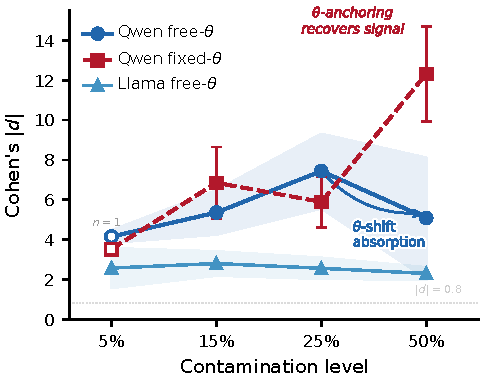
\includegraphics[width=\columnwidth]{fig_dose_response.pdf}
  \caption{Dose-response trajectories on MMLU. Free-$\theta$ (solid) shows non-monotonic behavior for Qwen due to $\theta$-shift absorption (shaded); fixed-$\theta$ (dashed) removes the inverted-U artifact and yields an overall positive dose-response ($|d|{=}12.32$ at 50\%). Llama's flat trajectory reflects minimal absorption. Hollow markers: single-seed ($n{=}1$); error bars: $\pm$SD ($n{=}3$).}
  \label{fig:dose_response}
\end{figure}

\subsection{$\Delta\ell_z^*$ Matched-Difference Design}
\label{sec:did}

LLM response patterns systematically violate IRT assumptions of local independence and unidimensionality.
In our empirical data, 57 of 60 model-benchmark cells yield $|\ell_z^*| > 1.96$ even absent contamination, rendering absolute thresholds uninformative.
We address this through a matched-difference design.

For controlled experiments with clean baselines, we compute:
\begin{equation}
  \Delta\ell_z^* = \ell_{z,\text{contam}}^{*} - \bar{\ell}_{z,\text{clean}}^{*}
  \label{eq:delta_lz}
\end{equation}
where $\bar{\ell}_{z,\text{clean}}^{*}$ averages over $n{=}10$ clean seeds.
The shared model misfit cancels, isolating contamination-specific aberrance.
We quantify effect sizes as $d = (\ell_{z,\text{contam}}^{*} - \bar{\ell}_{z,\text{clean}}^{*})\,/\,s_{\text{clean}}$, where $s_{\text{clean}}$ is the SD of the $n{=}10$ clean-seed $\ell_z^*$ values; with a single contaminated observation per condition, $d$ is a standardized departure rather than a two-sample effect size (Hedges' $g = J \cdot d$, $J \approx 0.914$ for $n{=}10$; \citealp{hedges1981}).
We report percentile bootstrap 95\% CIs (10,000 resamples) reflecting clean-seed variability only; bias-corrected and accelerated (BCa) correction (Appendix~\ref{app:bca}) generally confirms conservative coverage; multi-seed contamination-run variance appears in Appendix~\ref{app:reproducibility}.

For deployment without clean baselines, cross-benchmark comparison provides the reference: the target benchmark's $\ell_z^*$ is compared against benchmarks presumed clean from the same model.
Significance thresholds derive from a nonparametric bootstrap null rather than the asymptotic $\mathcal{N}(0,1)$ reference, accommodating residual model misspecification.
Simulation analysis (Appendix~\ref{app:local_dep}) confirms that the matched-difference design is robust to local dependence at realistic levels ($d_{\text{ratio}} \geq 0.93$ for $\sigma_\tau \leq 0.5$) and maintains ${\geq}98.5\%$ power even under contamination-specific asymmetric dependence.

\subsection{Experimental Setup}
\label{sec:setup}

\paragraph{Models and contamination.}
We validate on three 7--8B model families: Qwen2.5-7B-Instruct, Llama-3.1-8B-Instruct, and Mistral-7B-Instruct-v0.3.
Each is fine-tuned with Quantized Low-Rank Adaptation (QLoRA; rank\,$=$\,16, $\alpha$\,$=$\,32; full hyperparameters in Appendix~\ref{app:hyperparams}) under clean and contaminated conditions at varying levels: at $X\%$ contamination, $X\%$ of SFT training examples are benchmark items (questions paired with gold answers in the standard evaluation format), with the remainder drawn from a general instruction-following dataset.
All three families are tested at 15\% and 50\% contamination.
Following initial observation of non-monotonic dose-response for Qwen, we added 5\% and 25\% conditions for Qwen to trace the full dose-response curve.
Both conditions were subsequently extended to Llama to test whether the pattern generalizes; Mistral was additionally tested at 5\% but not at 25\% due to computational constraints.
We train $n{=}10$ independent clean seeds per model to establish baseline variability and construct bootstrap confidence intervals.
Reported CIs reflect variability across $n$ clean baseline seeds; for each model family, selected contamination levels were additionally replicated with $n{=}3$ independent QLoRA seeds to assess training-run variance: Qwen at 15\%/25\%/50\%, Llama at 5\%/15\%/25\%/50\%, and Mistral at 5\%/15\%/50\% (Appendix~\ref{app:reproducibility}).

\paragraph{Benchmarks.}
We evaluate on MMLU \citep{hendrycks2021mmlu} (14,042 items) and ARC-Challenge \citep{clark2018arc} (295 PSN-IRT-calibrated items), spanning two orders of magnitude in benchmark size.
All 4PL item parameters are from \citet{psnirt2026}.
ARC-Challenge experiments were conducted on Qwen only, as the primary evaluation of cross-benchmark generalizability; extending to additional families was constrained by computational budget.

\paragraph{Post-RL extension.}
To probe behavior boundaries beyond SFT, we apply Group Relative Policy Optimization (GRPO; \citealp{shao2024}) to one contaminated Qwen model (15\% MMLU) for 1,500 steps, evaluating at three checkpoints.
This extension is $N{=}1$ (single model family, single contamination level).

\paragraph{Evaluation protocol.}
Ability estimation uses maximum likelihood (MLE) with Newton--Raphson optimization on the 4PL log-likelihood.
For each model, we compute $\ell_z^*$ on the full benchmark response vector; seen/unseen decomposition recomputes $\ell_z^*$ on item subsets to localize the contamination signal.
All evaluations use greedy decoding (temperature~0) with the standard multiple-choice prompt format from the lm-evaluation-harness \citep{eval-harness}.

\paragraph{Contamination model.}
QLoRA SFT on benchmark items proxies SFT-stage contamination, analogous to a test-taker with item preknowledge.
At each contamination level, contaminated items are shuffled into the training mixture and presented in the same question--answer format used during evaluation, maximizing the memorization signal.
We term contaminated items \emph{seen} and the remainder \emph{unseen}, enabling person-fit decomposition (\S\ref{sec:degradation}).
Findings are scoped to SFT-based contamination.
